\documentclass[journal]{IEEEtran}
\IEEEoverridecommandlockouts

\usepackage{amsmath}
\usepackage{amssymb}
\usepackage{booktabs}
\usepackage{graphicx}
\usepackage{url}
\usepackage{cite}

\def\BibTeX{{\rm B\kern-.05em{\sc i\kern-.025em b}\kern-.08em
    T\kern-.1667em\lower.7ex\hbox{E}\kern-.125emX}}

\begin{document}

\title{Transfer Learning Across ECG Domains: PTB-XL Morphology Encoders on Chapman-Shaoxing Rhythm Classification}

\author{
    \IEEEauthorblockN{Lina Mar\'ia Casta\~neda C\'ardenas,
    \'Angel Cruz-Roa}\\
    \IEEEauthorblockA{\textit{Facultad de Ciencias B\'asicas e Ingenier\'ia (FCBI)},
    Universidad de los Llanos, Villavicencio, Colombia}\\
    \IEEEauthorblockA{macardenas@unillanos.edu.co, aacruz@unillanos.edu.co}
}

\maketitle

\begin{abstract}
Electrocardiogram (ECG) classification models trained on one dataset often fail to generalize across populations and clinical tasks. This work investigates cross-domain transfer learning between two heterogeneous ECG datasets: PTB-XL, a European multi-label morphology dataset, and Chapman-Shaoxing, a Chinese multiclass rhythm dataset. Three deep learning architectures---a 1D ResNet, a CNN-LSTM hybrid, and an ECG Transformer---were trained on PTB-XL for morphological superclass detection and evaluated as frozen encoders on Chapman-Shaoxing rhythm classification via linear probing. Results show that all encoders transfer above chance, with the CNN-LSTM achieving the highest cross-domain F1 macro of 0.674, compared to 0.503 for the ResNet and 0.485 for the Transformer, versus baselines of approximately 0.946 when trained from scratch on Chapman-Shaoxing. The CNN-LSTM advantage is attributed to its sequential temporal modeling, which captures rhythm-relevant dependencies not encoded by purely morphological or global-attention approaches. These findings suggest that temporal representations learned from morphology tasks partially generalize to rhythm classification, and that architecture choice critically determines transfer effectiveness across ECG domains.
\end{abstract}

\section{Introduction}

Cardiovascular diseases (CVD) remain a leading cause of mortality worldwide, and the electrocardiogram (ECG) is the primary non-invasive tool for their detection \cite{who2021cvd}. Deep learning models have demonstrated cardiologist-level performance on ECG classification tasks \cite{hannun2019cardiologist}, yet most systems are trained and evaluated within a single dataset, limiting their clinical applicability across institutions and populations.

Two fundamental challenges arise in cross-domain ECG learning. First, datasets differ in population demographics: PTB-XL \cite{wagner2020ptbxl} comprises European patients while Chapman-Shaoxing \cite{zheng2020chapman} comprises Chinese patients, introducing distributional shifts in signal morphology. Second, datasets encode clinically distinct information: PTB-XL labels morphological superclasses such as myocardial infarction (MI) and ST/T-wave changes (STTC), whereas Chapman-Shaoxing labels cardiac rhythms such as atrial fibrillation (AFIB) and sinus bradycardia (SB). These axes of classification are clinically orthogonal, making cross-domain transfer non-trivial. PTB-XL and Chapman-Shaoxing represent two of the largest and most widely used public ECG benchmarks \cite{wagner2020ptbxl, zheng2020chapman}, making them natural candidates for evaluating cross-domain generalization.

Transfer learning from large source datasets has been widely studied in medical imaging \cite{raghu2019transfusion}, but cross-dataset ECG transfer---particularly across clinically heterogeneous tasks---remains underexplored. Prior work has shown that pre-training on large ECG corpora improves downstream performance \cite{mehari2022selfsupervised}, but the role of architecture in determining transfer effectiveness has received limited attention \cite{strodthoff2021ptbxl}.

This paper addresses the following question: \textit{how much do ECG representations learned for morphology classification transfer to rhythm classification across heterogeneous populations, and which architecture transfers most effectively?} We additionally evaluate whether incorporating demographic clinical variables (age and sex) at the classifier head improves performance on the source domain. Our contributions are: (1) a systematic cross-domain linear probing evaluation of three architectures across two clinically and demographically distinct ECG datasets; (2) evidence that sequential temporal encoders (CNN-LSTM) transfer significantly better than morphological (CNN ResNet) or global-attention (Transformer) encoders to rhythm classification; and (3) an analysis of demographic variable integration showing no consistent improvement over ECG signal alone.

\section{Methods}

\subsection{Datasets}

\textbf{PTB-XL} \cite{wagner2020ptbxl} is a publicly available 12-lead ECG dataset of 21,799 recordings from European patients at 100\,Hz and 500\,Hz. Each recording is annotated with SCP codes mapped to five diagnostic superclasses: Normal (NORM), Myocardial Infarction (MI), ST/T-wave Changes (STTC), Conduction Disturbance (CD), and Hypertrophy (HYP). Following the official protocol \cite{wagner2020ptbxl}, recordings with confidence below 50\% were excluded, yielding 20,373 labeled samples. The task is multi-label binary classification using BCEWithLogitsLoss with per-class positive weights. The official stratified fold split was used: folds 1--8 for training, fold 9 for validation, and fold 10 for test.

\textbf{Chapman-Shaoxing} \cite{zheng2020chapman} comprises 10,646 12-lead ECG recordings from Chinese patients at 500\,Hz. Eleven original rhythm annotations were grouped into four classes following \cite{zheng2020chapman}: AFIB (atrial fibrillation and flutter), GSVT (supraventricular tachycardias), SB (sinus bradycardia), and SR (sinus rhythm and sinus irregularity). Signals were resampled to 100\,Hz using polyphase filtering and cropped to 9\,s (900 samples) after removing filter transient edges. The task is single-label multiclass classification using CrossEntropyLoss with class weights. A 70/10/20 stratified split was used for training, validation, and test.

\subsection{Architectures}

Three architectures were implemented for PTB-XL and adapted for Chapman-Shaoxing:

\textbf{CNN1D-ResNet} \cite{he2016resnet}: A 1D residual network with an input convolutional stem (kernel 15, MaxPool $\times$2), four residual blocks with progressive channel expansion (64$\to$128$\to$256), Global Average Pooling, and a projection layer to a 128-dimensional latent space. Approximately 1.7M parameters.

\textbf{CNN-LSTM}: A hybrid architecture combining a three-stage CNN feature extractor (12$\to$64$\to$128$\to$256 channels, three MaxPool$\times$2) with a two-layer bidirectional LSTM (hidden size 256, effective output 512-d), temporal max-pooling readout, and a linear projection to 128-d. Approximately 5.2M parameters. The max-pooling readout replaces the commonly used last hidden state, improving stability by capturing the strongest activation across all temporal positions \cite{sun2024cnnlstm, mahajan2025graph}.

\textbf{ECG Transformer}: A patch-based Transformer encoder \cite{islam2024ecgformer} with a lightweight CNN stem, patch size 50 (20 patches per 1000-sample signal), learned positional encoding, a [CLS] classification token, two Transformer encoder blocks \cite{vaswani2017attention} ($d_{model}=256$, 8 heads, MLP ratio 4), and a 128-d projection head. Approximately 2.1M parameters. Dropout 0.3 and weight decay $5\times10^{-2}$ were applied to address overfitting observed in a four-layer variant.

All encoders terminate in a 128-dimensional projection layer (\texttt{get\_embeddings()}), enabling architecture-agnostic transfer. For PTB-XL, a linear head $\mathbb{R}^{128} \to \mathbb{R}^{5}$ is appended; for Chapman-Shaoxing trained from scratch, $\mathbb{R}^{128} \to \mathbb{R}^{4}$.

\subsection{Clinical Variable Integration}

To evaluate the contribution of demographic information, a second set of PTB-XL experiments concatenated normalized age (divided by 100) and binary sex encoding to the 128-d embedding before the classification head, yielding a 130-d input: $\mathbb{R}^{130} \to \mathbb{R}^{5}$.

\subsection{Transfer Learning Protocol}

Cross-domain transfer was performed via \textit{linear probing} \cite{chen2024patchecg}: each PTB-XL encoder was loaded from its best checkpoint, all parameters were frozen (\texttt{requires\_grad=False}), and a new linear head $\mathbb{R}^{128} \to \mathbb{R}^{4}$ was trained exclusively on Chapman-Shaoxing 100\,Hz embeddings. Embeddings were extracted once per split (deterministic under \texttt{eval()} and \texttt{no\_grad()}), and only the head was optimized using Adam ($lr=10^{-3}$), CrossEntropyLoss with Chapman class weights, and early stopping (patience 10) on validation F1 macro.

\subsection{Training Configuration}

All models were trained with Adam optimizer, gradient clipping (max norm 1.0), and early stopping. PTB-XL models used BCEWithLogitsLoss with per-class positive weights; Chapman models used CrossEntropyLoss with class weights. The ECG Transformer used AdamW with OneCycleLR scheduling. All experiments ran on an NVIDIA RTX 5050 (8\,GB VRAM) with batch size 128.

\section{Results}

\subsection{PTB-XL: Source Domain Performance}

Table~\ref{tab:ptbxl} reports test-set AUC macro and F1 macro for the three architectures on PTB-XL, with and without demographic variables. The CNN1D-ResNet achieves the highest AUC (0.918) and F1 (0.704). These results are consistent with the PTB-XL benchmark reported by Strodthoff et al.\ \cite{strodthoff2021ptbxl}, where ResNet-based architectures achieve macro AUC of 0.919--0.925 on the diagnostic superclass task. The CNN-LSTM follows closely (AUC 0.913, F1 0.695), while the ECG Transformer lags behind (AUC 0.898, F1 0.671), consistent with its smaller capacity (2.1M vs. 5.2M parameters) and the limited training set size ($\sim$16k samples).

Incorporating age and sex did not improve performance consistently across models or classes. The ResNet showed a decrease in F1 ($-$0.024), while the CNN-LSTM showed negligible change ($-$0.002) and the Transformer a slight decrease ($-$0.013). Notably, HYP---the class most expected to benefit from demographics---did not improve in the ResNet ($-$0.041) despite prior clinical evidence linking hypertrophy to age and sex. This suggests that ECG signal morphology already encodes sufficient demographic information implicitly.

\begin{table}[t]
\caption{PTB-XL test results (fold 10). AUC macro and F1 macro with and without demographic variables (age, sex).}
\label{tab:ptbxl}
\centering
\begin{tabular}{lcccc}
\toprule
\textbf{Model} & \multicolumn{2}{c}{\textbf{w/o clinical}} & \multicolumn{2}{c}{\textbf{w/ clinical}} \\
 & AUC & F1 & AUC & F1 \\
\midrule
CNN1D-ResNet   & 0.918 & 0.704 & 0.916 & 0.680 \\
CNN-LSTM       & 0.913 & 0.695 & 0.914 & 0.693 \\
ECGTransformer & 0.898 & 0.671 & 0.895 & 0.658 \\
\bottomrule
\end{tabular}
\end{table}

\subsection{Chapman-Shaoxing: Target Domain Performance}

Table~\ref{tab:transfer} presents the main result of this work. All three models achieve high accuracy ($>$0.94 F1 macro) when trained from scratch on Chapman-Shaoxing, confirming that the rhythm classification task is well-suited to all three architectures given sufficient in-domain data. These results align with prior work on Chapman-Shaoxing, where Inception-v3 based models achieve F1 of 0.952 \cite{hong2022bimodal} and CNN-BiLSTM architectures report competitive performance \cite{mahajan2025graph}.

\begin{table}[t]
\caption{Chapman-Shaoxing 100\,Hz test results. Scratch: trained from scratch. Transfer: PTB-XL encoder frozen, only linear head trained on Chapman.}
\label{tab:transfer}
\centering
\begin{tabular}{lcccc}
\toprule
\textbf{Model} & \multicolumn{2}{c}{\textbf{Scratch}} & \multicolumn{2}{c}{\textbf{Transfer}} \\
 & Acc & F1 & Acc & F1 \\
\midrule
CNN1D-ResNet   & 0.952 & 0.947 & 0.515 & 0.503 \\
CNN-LSTM       & 0.951 & 0.946 & 0.687 & 0.674 \\
ECGTransformer & 0.948 & 0.943 & 0.499 & 0.485 \\
\bottomrule
\end{tabular}
\end{table}

\begin{figure}[t]
\centering
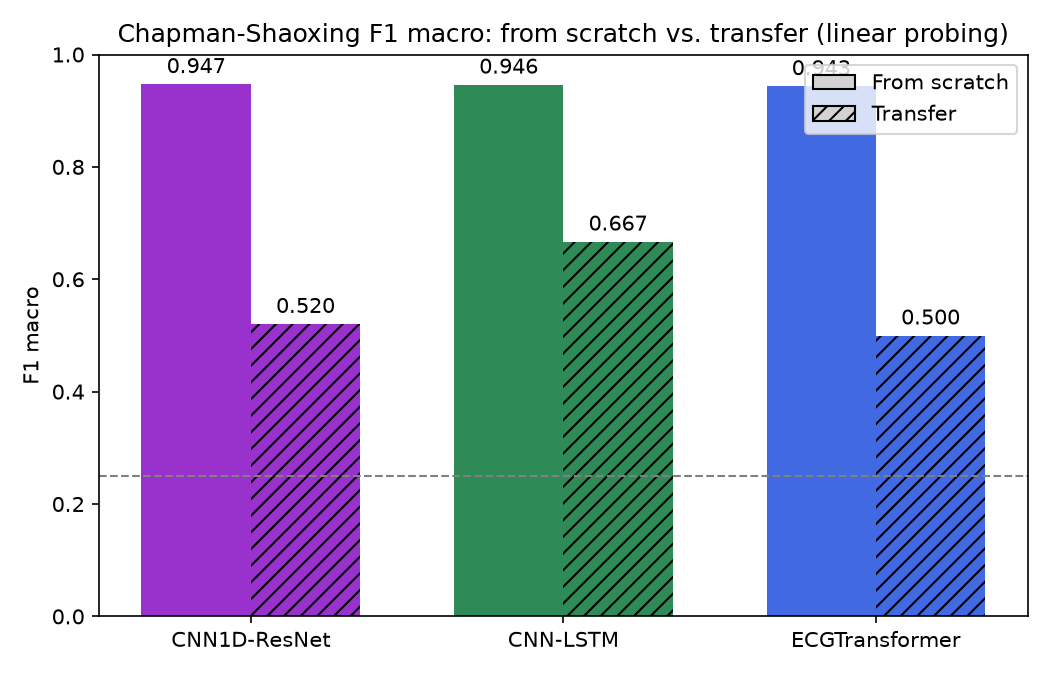
\includegraphics[width=\columnwidth]{fig2_scratch_vs_transfer.png}
\caption{F1 macro on Chapman-Shaoxing: models trained from scratch vs.\
frozen PTB-XL encoders (linear probing). Dashed line indicates chance
level (0.25).}
\label{fig:scratch_vs_transfer}
\end{figure}

\begin{figure}[t]
\centering
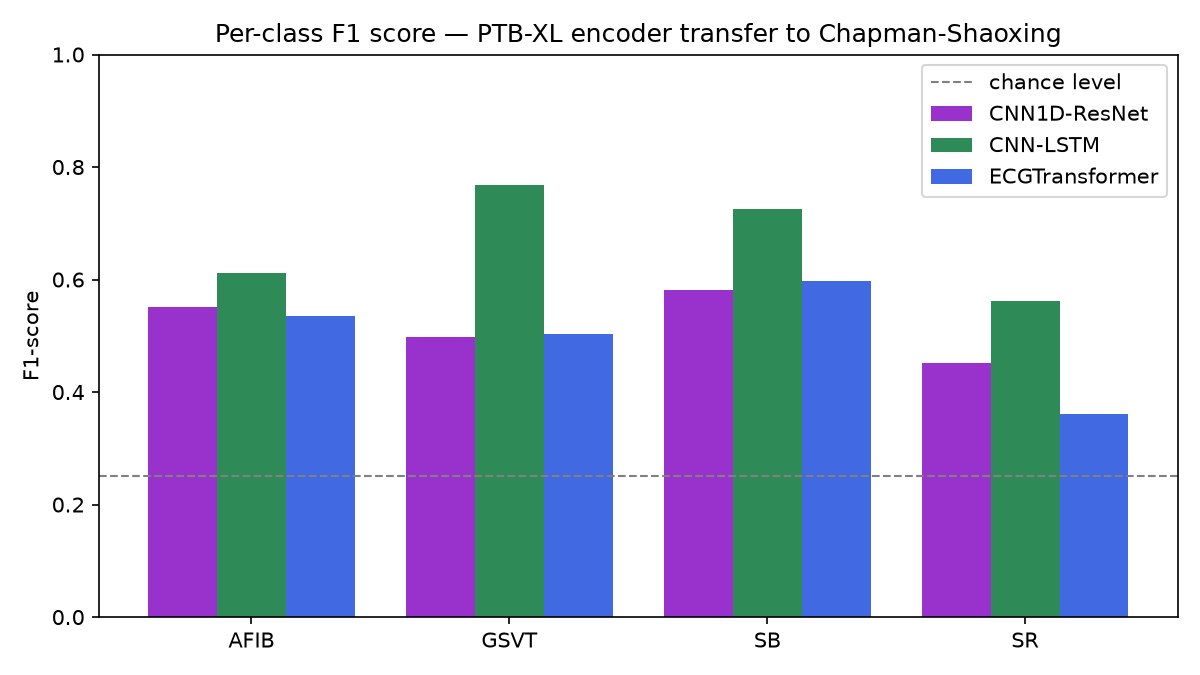
\includegraphics[width=\columnwidth]{fig1_transfer_by_class.png}
\caption{Per-class F1 under linear probing transfer from PTB-XL to
Chapman-Shaoxing. SB transfers most consistently; SR transfers least
across all encoders.}
\label{fig:transfer_by_class}
\end{figure}

Three key findings emerge from Table~\ref{tab:transfer} and
Figs.~\ref{fig:scratch_vs_transfer}--\ref{fig:transfer_by_class}.
First, the CNN-LSTM encoder achieves the highest transfer F1 of 0.674,
outperforming the CNN1D-ResNet (0.503) and ECGTransformer (0.485) by
16--19 percentage points---a gap too large to attribute to random
variation. Second, all three encoders transfer well above the
four-class chance level of 0.25, confirming that PTB-XL morphology
encoders capture genuinely useful structure for rhythm classification,
even without any Chapman-Shaoxing data during encoder training. Third,
when trained from scratch on Chapman-Shaoxing, the three architectures
converge to near-identical F1 scores (0.943--0.947), indicating that
architecture choice matters far less than data availability in the
target domain.

Table~\ref{tab:transfer_per_class} details per-class F1 scores under
transfer, complementing Fig.~\ref{fig:transfer_by_class}. The CNN-LSTM
achieves the strongest results across all four rhythm classes, with a
particularly large advantage on GSVT (0.770 vs.\ 0.474 and 0.511) and
SB (0.745 vs.\ 0.580 and 0.560). SR remains the hardest class to
transfer for all encoders, with the ECGTransformer reaching only 0.348.

\begin{table}[t]
\caption{Per-class F1 score under linear probing transfer
(PTB-XL encoder $\to$ Chapman-Shaoxing 100\,Hz test set).}
\label{tab:transfer_per_class}
\centering
\begin{tabular}{lcccc}
\toprule
\textbf{Model} & \textbf{AFIB} & \textbf{GSVT} & \textbf{SB} & \textbf{SR} \\
\midrule
CNN1D-ResNet   & 0.545 & 0.474 & 0.580 & 0.414 \\
CNN-LSTM       & 0.616 & 0.770 & 0.745 & 0.566 \\
ECGTransformer & 0.530 & 0.511 & 0.560 & 0.348 \\
\bottomrule
\end{tabular}
\end{table}

\section{Discussion}

The central scientific question of this work is whether a model trained
exclusively on European ECG morphology (PTB-XL: NORM, MI, STTC, CD, HYP)
can generalize to rhythm classification in Chinese ECG signals
(Chapman-Shaoxing: AFIB, GSVT, SB, SR) without ever observing
Chapman-Shaoxing data during encoder training. Our linear probing
experiment---where PTB-XL encoders are fully frozen and only a single
linear head is trained on Chapman-Shaoxing---provides a controlled
answer: yes, but the degree of transfer depends critically on
architecture.

The CNN-LSTM encoder transfers substantially better (F1 0.674) than
the CNN1D-ResNet (F1 0.503) or ECG Transformer (F1 0.485). We attribute
this to the nature of the representations each architecture learns. The
CNN1D-ResNet specializes in local morphological patterns---P-wave shape,
QRS complex, T-wave amplitude---which are highly specific to the
PTB-XL superclasses and do not generalize well to rhythm. The ECG
Transformer, despite its global attention mechanism, appears to
concentrate its [CLS] token representation toward source-domain
morphological features, limiting cross-domain utility. In contrast, the
CNN-LSTM's bidirectional LSTM models inter-beat sequential
dependencies---RR interval regularity, rhythm periodicity,
beat-to-beat variability---which are precisely the features that
distinguish the four Chapman-Shaoxing rhythm classes. This finding
has a direct clinical interpretation: \textit{sequential temporal
representations learned from morphology tasks partially encode
rhythm-relevant structure, while purely morphological or global-attention
representations do not}.

Among rhythm classes, SB (sinus bradycardia) transfers most
consistently across all encoders (F1: 0.580, 0.745, 0.560 for ResNet,
LSTM, Transformer respectively), while SR (sinus rhythm) transfers
least (F1: 0.414, 0.566, 0.348). Bradycardia is characterized by
globally prolonged RR intervals and slower overall signal morphology,
leaving detectable traces in morphological encoders trained on PTB-XL.
Normal sinus rhythm, being the default cardiac pattern, is harder to
distinguish from morphological features alone and likely requires
rhythm-specific temporal context to classify reliably.

The failure of demographic variables (age and sex) to improve PTB-XL
performance is a secondary but relevant finding. Contrary to the
expectation that clinical metadata would benefit morphologically
correlated classes such as HYP (hypertrophy), adding age and sex
reduced F1 in the CNN1D-ResNet ($-$0.024) and ECGTransformer
($-$0.013), with negligible change in the CNN-LSTM ($-$0.002). This
suggests that well-trained ECG encoders implicitly capture
age- and sex-correlated morphological patterns from the signal itself,
rendering explicit demographic features redundant or mildly disruptive.

\textbf{Limitations and future work.} Linear probing represents a
lower bound on transfer performance; fine-tuning the encoder on
Chapman-Shaoxing data would likely reduce the gap substantially,
and future work should quantify this improvement. Only 100\,Hz
signals were used for cross-domain experiments to maintain frequency
consistency with PTB-XL; evaluating at 500\,Hz remains an open
direction. The transfer gap also motivates exploring contrastive
pre-training strategies \cite{mehari2022selfsupervised} that
explicitly align representations across domains, as well as
domain adaptation techniques \cite{niu2020domain} that do not require target labels.
Finally, extending this evaluation to additional datasets across
diverse populations would strengthen the generalizability of
the findings reported here.

\section{Conclusion}

We investigated whether ECG morphology representations learned on
PTB-XL (European, multi-label) transfer to rhythm classification on
Chapman-Shaoxing (Chinese, multiclass) via linear probing across three
deep learning architectures. The CNN-LSTM encoder transfers
significantly better (F1 0.674) than the CNN1D-ResNet (F1 0.503) or
ECG Transformer (F1 0.485), demonstrating that sequential temporal
modeling captures rhythm-relevant structure that purely morphological
or global-attention approaches do not encode. All encoders transfer
above chance, confirming that cross-domain ECG transfer is feasible
even across clinically orthogonal tasks and demographically distinct
populations. When trained from scratch, all three architectures achieve
equivalent performance on Chapman-Shaoxing (F1 $\approx$ 0.945),
indicating that architecture matters primarily when in-domain data is
scarce. These results highlight architecture selection as a critical
factor in cross-domain ECG transfer and motivate future work on
fine-tuning and domain adaptation for heterogeneous clinical datasets.

\section*{Acknowledgment}
The authors thank the Universidad de los Llanos for institutional support.

\begin{thebibliography}{00}

\bibitem{who2021cvd}
World Health Organization, ``Cardiovascular diseases (CVDs),'' Fact sheet, 2021. [Online]. Available: \url{https://www.who.int/news-room/fact-sheets/detail/cardiovascular-diseases-(cvds)}

\bibitem{hannun2019cardiologist}
A. Y. Hannun \textit{et al.}, ``Cardiologist-level arrhythmia detection and classification in ambulatory electrocardiograms using a deep neural network,'' \textit{Nature Medicine}, vol. 25, no. 1, pp. 65--69, 2019.

\bibitem{wagner2020ptbxl}
P. Wagner \textit{et al.}, ``PTB-XL, a large publicly available electrocardiography dataset,'' \textit{Scientific Data}, vol. 7, no. 1, p. 154, 2020.

\bibitem{zheng2020chapman}
J. Zheng \textit{et al.}, ``A 12-lead electrocardiogram database for arrhythmia research covering more than 10,000 patients,'' \textit{Scientific Data}, vol. 7, no. 1, p. 48, 2020.

\bibitem{he2016resnet}
K. He, X. Zhang, S. Ren, and J. Sun, ``Deep residual learning for image recognition,'' in \textit{Proc. IEEE CVPR}, 2016, pp. 770--778.

\bibitem{raghu2019transfusion}
M. Raghu, C. Zhang, J. Kleinberg, and S. Bengio, ``Transfusion: Understanding transfer learning for medical imaging,'' in \textit{Proc. NeurIPS}, 2019, pp. 3347--3357.

\bibitem{mehari2022selfsupervised}
T. Mehari and N. Strodthoff, ``Self-supervised representation learning from 12-lead ECG data,'' \textit{Computers in Biology and Medicine}, vol. 141, p. 105114, 2022.

\bibitem{islam2024ecgformer}
M. Islam \textit{et al.}, ``ECGformer: Leveraging transformer for ECG arrhythmia detection,'' \textit{arXiv preprint arXiv:2401.05434}, 2024.

\bibitem{sun2024cnnlstm}
Y. Sun \textit{et al.}, ``CNN-LSTM with squeeze-and-excitation for ECG arrhythmia classification,'' \textit{Sensors}, vol. 24, no. 6, p. 2406306, 2024.

\bibitem{vaswani2017attention}
A. Vaswani \textit{et al.}, ``Attention is all you need,'' in \textit{Proc. NeurIPS}, 2017, pp. 5998--6008.

\bibitem{strodthoff2021ptbxl}
N. Strodthoff, P. Wagner, T. Schaeffter, and W. Samek, ``Deep learning
for ECG analysis: Benchmarks and insights from PTB-XL,'' \textit{IEEE
J. Biomed. Health Inform.}, vol. 25, no. 5, pp. 1519--1528, 2021.

\bibitem{niu2020domain}
L. Niu \textit{et al.}, ``A deep-learning approach to ECG classification
based on adversarial domain adaptation,'' \textit{Healthcare}, vol. 8,
no. 4, p. 437, 2020.

\bibitem{chen2024patchecg}
M. Chen \textit{et al.}, ``PatchECG: Masked patch modelling for
self-supervised ECG representation learning,'' \textit{Scientific
Reports}, 2024.

\bibitem{mahajan2025graph}
P. Mahajan and A. Kaul, ``Graph-enhanced deep learning for ECG
arrhythmia detection: An integration of CNN, GNN, and BiLSTM,''
\textit{Medical Engineering and Physics}, vol. 145, p. 104418, 2025.

\bibitem{hong2022bimodal}
S. Hong \textit{et al.}, ``Bimodal CNN for cardiovascular disease
classification by co-training ECG grayscale images,'' \textit{Scientific
Reports}, 2022.

\end{thebibliography}

\end{document}
